\Chapter{Tesztelés}

A fejezetben be kell mutatni, hogy az elkészült alkalmazás hogyan használható.
(Az, hogy hogyan kell, hogy működjön, és hogy hogy lett elkészítve, az előző fejezetekben már megtörtént.)

Jellemzően az alábbi dolgok kerülhetnek ide.
\begin{itemize}
\item Tesztfuttatások. Le lehet írni a futási időket, memória és tárigényt.
\item Felhasználói kézikönyv jellegű leírás. Kifejezetten a végfelhasználó szempontjából lehet azt bemutatni, hogy mit hogy lehet majd használni.
\item Kutatás kapcsán ide főként táblázatok, görbék és egyéb részletes összesítések kerülhetnek.

\end{itemize}

\textbf{Teszt}


A program megvalósításához szóba jött a Jquerry használata is, és ezáltal az is, hogy vajon a Jquerry-s vagy a sima context-re rajzolás lehet-e a gyorsabb.

Ehhez a vizsgálathoz két példa program is készült, az egyik azt vizsgálta, hogy melyik megoldás milyen gyorsasággal rajzol ki. 

1000-től 29000-ig vizsgáltuk a kirajzolást ezresével növelve a méretet, ugyanazzal a kitöltéssel, mérettel, és már itt láttuk, hogy a Jquerry sokkal lassabb. Az itt kapott futási időket \Aref{fig:pieces}. grafikon tartalmazza. 

\begin{figure}[h]
	\centering
	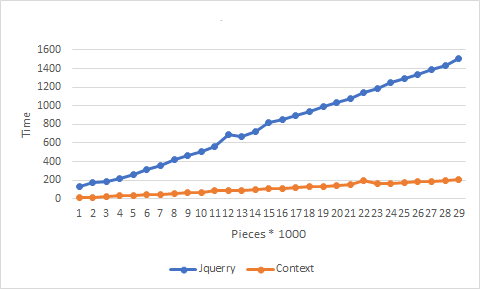
\includegraphics[scale=1]{images/pieces.png}
	\caption{Jquerry vs context kirajzolás daraszám alapján.}
	\label{fig:pieces}
\end{figure}


De vizsgáltunk egy másik szempontot is, még pedig, hogy ha a körök méretét növeljük, akkor melyik a gyorsabb. 

10-től 290-es méretig rajzoltattunk ki köröket tizesével növelve a méretet, és itt is láthattuk, hogy a Jquerry lassabb, így a programban azt a megoldást nem használtuk. Az itt kapott futási időket pedig \Aref{fig:radius}. grafikon tartalmazza

\begin{figure}[h]
	\centering
	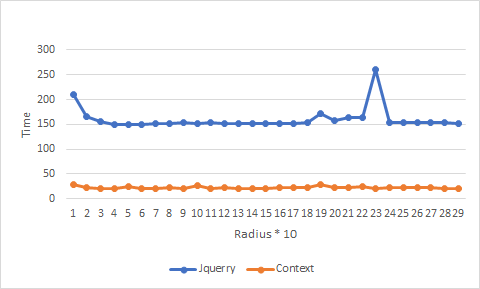
\includegraphics[scale=1]{images/radius.png}
	\caption{Jquerry vs context kirajzolás méret alapján.}
	\label{fig:radius}
\end{figure}
